\chapter{Equazioni differenziali ordinarie}
\section{Introduzione alle \odes}
\begin{definition} \label{Def: ODE}
Si dice \textbf{equazione differenziale ordinaria} di ordine $n$ un'equazione funzionale della forma
\begin{equation}
    F\left(x, y(x), y'(x), \dots, y^{(n)}(x)\right)=0
\end{equation}
dove  $F:A \subseteq \R^{n+2} \to \R$, $y=y(x)$ è l'incognita e $x$ è la variabile indipendente.
\end{definition}
\begin{oss}
    Solitamente $F$ è una funzione continua.
\end{oss}
\begin{oss}
    È abbastanza frequente l'omissione della variabile indipendente nella scrittura dell'equazione.
\end{oss}
\begin{definition} \label{Def: ODE in forma normale}
    Un'\ode si dice in \textbf{forma normale} se è del tipo
    \begin{equation}
        y^{(n)}(x)=f\left(x, y(x), y'(x), \dots, y^{(n-1)}(x)\right)
    \end{equation}
    con $f:A\subseteq \R^{n+1} \to \R$, $A$ aperto.
\end{definition}
\begin{definition} \label{Def: Soluzione di un'ode}
    Si dice \textbf{soluzione} o \textbf{integrale} dell'\ode su un certo $I\subseteq \R$ una funzione $\varphi: I \to \R$ derivabile $n$ volte su $I$ tale che 
    \begin{equation}
         F\left(x, \varphi(x), \varphi'(x), \dots, \varphi^{(n)}(x)\right)=0 \qquad \forall\ x \in I
    \end{equation}
\end{definition}
\begin{example}
    Si prenda la seguente equazione in forma normale di ordine 1: 
    \begin{equation*}
        y'(x)=y(x)
    \end{equation*}
    Essa è verificata in ogni $x \in \R$ dalla funzione $\varphi(x)= e^x$.
\end{example}
Oltre a parlare di equazioni differenziali ordinarie, si può parlare di sistemi di equazioni differenziali ordinarie di ordine $n$.
\begin{definition} \label{Def: Sistema di ode del primo ordine}
    Si dice \textbf{sistema di \odes del primo ordine} un sistema di equazioni del tipo
    \begin{equation}
        \left\{
        \begin{aligned}
        y_1'(x) &= f_1(x, y_1, \dots, y_n)\\
         y_2'(x) &= f_2(x, y_1, \dots, y_n)\\       
        &\vdots \\
        y_n'(x) &= f_n(x, y_1, \dots, y_n)
        \end{aligned} \right.
\end{equation}
o, in forma compatta, 
\begin{equation}
    Y'=G(x, Y)
\end{equation}
con $Y: I \subseteq \R \to \R^n,\ Y=(y_1, \dots, y_n)$ e $G:I \times \R^n \to \R^n,\ G(x, Y)=(f_1, \dots, f_n)$
\end{definition}
\begin{definition} \label{Def: Sistema di ode lineare}
    Un sistema di \odes del primo ordine si dice \textbf{lineare} se $G$ è lineare in $Y$.
\end{definition}
\begin{definition} \label{Def: Sistema/Ode autonoma}
    Un sistema di \odes del primo ordine o un'\ode di ordine $n$ si dicono \textbf{autonomi} se non è presente una dipendenza esplicita da x, cioè se $G=G(y)$.
\end{definition}
\begin{lemma}
    Un'\ode di ordine $n$ in forma normale è equivalente ad un sistema di \odes del primo ordine in $\R^n$.
\end{lemma}
\begin{proof}
    Sia
    \begin{equation}
  (E):\ y^{(n)}=f\left(x, y, y', \dots, y^{(n-1)}\right)
    \end{equation}
    e si pongano
    \begin{equation}
        \begin{aligned}
            Y_1(x)&:=y(x)\\
            Y_2(x)&:=y'(x)\\
            &\vdots\\
            Y_n(x)&:=y^{(n-1)}
        \end{aligned}
    \end{equation}
    Si può osservare che, preso $Y=(Y_1, \dots, Y_n)$, si ha
    \begin{equation}
      (S):\ Y'= \begin{cases}
            Y_1'&= y_2\\
            Y_2'&=y_3\\
            &\vdots\\
            Y_n'&\overset{(E)}{=}f\left(x, y, y', \dots, y^{(n-1)}\right)
        \end{cases}
    \end{equation}
    Definendo poi
    \begin{equation}
        G(x, Y) := \begin{pmatrix}
            y_1\\
            y_2\\
            \vdots\\
            f(x, y_1, \dots, y_n)
        \end{pmatrix}
    \end{equation}
    Si ha che, se $y$ soddisfa $E$, allora 
    \begin{equation}
        Y(x)=\begin{pmatrix}
            y_1(x)\\
            y_2(x)\\
            \vdots\\
            y_n(x)
        \end{pmatrix}
    \end{equation}
    soddisfa $Y'=G(x, Y)$. D'altra parte, se $Y$ soddisfa $Y'=G(x, Y)$, la sua prima componente $y_1(=y(x))$ soddisfa $E$.
\end{proof}
\begin{oss}
Un'\ode ha generalmente infinite soluzioni. Infatti, dette $g, G$ rispettivamente una funzione generica e una sua primitiva, si ha che
\begin{equation}
    y'= g(x) \Rightarrow y(x)= G(x)+c,\quad c \in \R
\end{equation}
\end{oss}
\section{Problema di Cauchy}
\begin{definition}
    Si dice \textbf{problema di Cauchy} associato ad un sistema S: Y'=G(x,Y) il sistema
    \begin{equation}
       (P): \begin{cases}
            Y'=G(x, Y)\\
            Y(x_0)=Y_0
        \end{cases}
    \end{equation}
    dove $Y(x_0)$ è detto \textbf{condizione iniziale}.
\end{definition}
Occorre osservare che in un problema del genere è necessario che $x_0 \in \R,\ y_0 \in \R^n$ siano noti.
\begin{lemma}[Formulazione integrale del problema di Cauchy] \label{Lemma: Formulazione integrale del problema di Cauchy}
    Sia $f: A \subseteq \R^{n+1} \to \R^n$ con $A$ aperto e $f$ continua. Siano poi $(x_0, y_0) \in A$ e $\delta>0$. Allora le seguenti affermazioni sono equivalenti
    \begin{enumerate}
        \item Esiste $y=y(x)$ derivabile in $[x_0-\delta, x_0+\delta]$ tale che 
        \begin{equation}
            (P): \begin{cases}
                y'(x)=f(x, y(x)) \qquad (E)\\
                y(x_0)=y_0 
            \end{cases}
            \qquad \forall\ x \in [x_0-\delta, x_0+\delta]
        \end{equation}
        \item Esiste $y=y(x)$ continua in $[x_0-\delta, x_0+\delta]$ tale che 
        \begin{equation} \label{Eq: Equazione integrale di Volterra}
            y(x)= y_0 + \int\limits_{x_0}^{x}{f(s, y(s))}\, ds \qquad \forall\ x \in [x_0-\delta, x_0+\delta]
        \end{equation}
    \end{enumerate}
\end{lemma}
\begin{proof}
    $1 \Rightarrow 2$: Sia $y$ come nelle ipotesi di $(1)$. Si integrino entrambi i membri di $(E)$ tra $x_0$ e $x \in [x_0-\delta, x_0+\delta]$. Allora
    \begin{equation}
        y(x)-y_0=\int\limits_{x_0}^{x}{f(s, y(s))}\,ds
    \end{equation}
    e $y$ è continua e soddisfa $(2)$.\\
    $2 \Rightarrow 1$: Sia $y$ come nelle ipotesi di $(2)$. Allora si ha che
    \begin{equation}
        y(x_0)=y(x)= y_0 + \int\limits_{x_0}^{x_0}{f(s, y(s))}\, ds= y_0
    \end{equation}
    Poi, $f(s, y(s))$ è continua per composizione di funzioni continue. Quindi dal TFC si ha che $y(x)$ è derivabile e
    \begin{equation}
        y'(x)= \left[y_0 + \int\limits_{x_0}^{x}{f(s, y(s))}\, ds\right]'= f(x, y(x)) \qquad \forall\ x \in [x_0-\delta, x_0+\delta]
    \end{equation}
    cioè che $y$ risolve il problema (P) di Cauchy.
\end{proof}
\begin{theorem}[Teorema di Peano dell'esistenza locale]
Si consideri il problema di Cauchy
\begin{equation}
    (P): \begin{cases}
        Y'=G(x, Y)\\
        Y(x_0)=Y_0
    \end{cases}
\end{equation}
Se $G \in C^0(B_\delta(x_0, y_0))$, allora esistono $\delta>0,\ \varphi$ tali che $\varphi: (x_0- \delta, x_0+\delta) \to \R^n$ sia soluzione di P.
\end{theorem}
Il teorema garantisce l'esistenza della soluzione ma non l'unicità.
\begin{example}
Si consideri il seguente problema di Cauchy.
\begin{equation*}
    (P):\begin{cases}
        y'=3y^{\frac{2}{3}}\\
        y(0)=0
    \end{cases}
\end{equation*}
Si può facilmente osservare che la soluzione costante $y=0$ è una soluzione del problema.\\
Un'altra soluzione può essere $y=x^3$, infatti
\begin{equation*}
    y(0)=0^3=0, \qquad y'(x)=3x^2=3(x^3)^\frac{2}{3}=3x^2
\end{equation*}
Allo stesso modo, si può mostrare che, fissati $a,\ b \in \R$ tali che $a<0<b$, la funzione
\begin{equation*}
y^*= \begin{cases}
    (x-a)^3 &\qquad x\leq a\\
    0 &\qquad a \leq x \leq b\\
    (x-b)^3 &\qquad x \geq b
\end{cases}
\end{equation*}
è anch'essa soluzione del problema di Cauchy.\\
Pertanto, le soluzioni del problema sono infinite e una loro rappresentazione grafica dà vita al cosiddetto \textit{pennello di Peano}.
\begin{figure}[H]
\centering
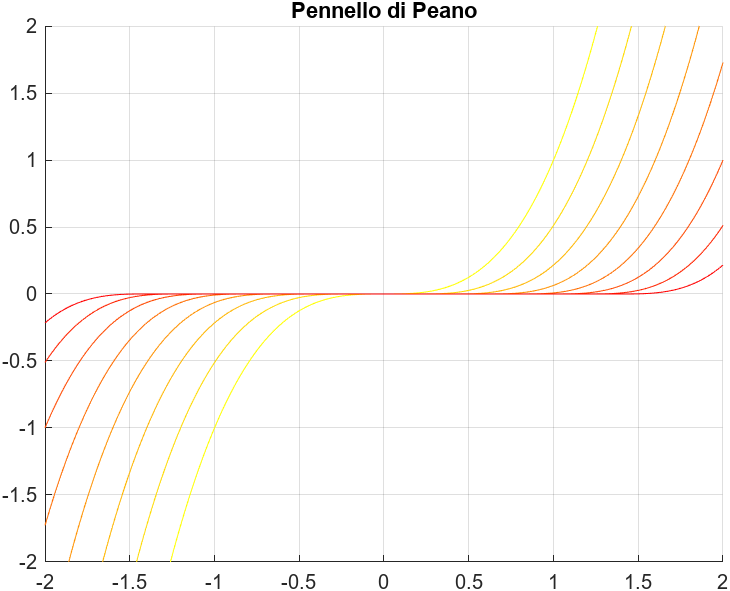
\includegraphics[width=0.31\textwidth]{Capitoli/Capitolo8/Pennello di Peano.png}
\end{figure}
\end{example}
D'altra parte, è anche vero che è possibile stabilire una condizione sufficiente per l'esistenza e unicità locale di un problema di Cauchy. Prima però bisogna definire il concetto di lipschitzianità locale (cfr. \ref{Def: Funzione lipschitziana}).
\begin{definition}
    Si dice che una funzione $G: A\subseteq \R^{n+1} \to \R^n$ con $A$ aperto è \textbf{localmente Lipschitziana} nell'insieme $A$ in $y$ uniformemente rispetto a $x$ se in ogni compatto $K \subset A$ esiste una costante di Lipschitz $L_K$ tale che
    \begin{equation}
        \forall\ (x, y_1), (x, y_2) \in K \ \text{si ha che}\ |G(x, y_1)-G(x, y_2)| \leq L_K |y_1-y_2|
    \end{equation}
\end{definition}
\begin{theorem}[Teorema di Cauchy di esistenza e unicità locale]
    Siano $A \subseteq \R^{n+1}$ aperto e $G:A \to \R^n$ continua, localmente Lipschitziana in $Y$ e uniformemente rispetto a $x$ in $B_\delta(x_0, y_0) \subset A$. Sia poi $(x_0, Y_0) \in A$. Allora esiste $\delta>0$ tale che il problema di Cauchy
    \begin{equation}
        (P): \begin{cases}
            Y'=G(x, Y)\\
            Y(x_0)=Y_0
        \end{cases}
    \end{equation}
    ammetta un'unica soluzione locale $\overline{Y}$ per $x \in [x_0-\delta, x_0+\delta]$
\end{theorem}
\begin{proof}
Siano $a, b>0$ tali che si possa definire $R \subseteq A$ come
\begin{equation}
    R= \{(x,y) \mid |x-x_0|\leq a, |y-y_0| \leq b \}
\end{equation}
Siano poi $L>0$ la costante di Lipschitz di $G$ su $R$ e 
\begin{equation}
M=\max\limits_{R}{|G(x, y)|} \qquad 0<\delta<\min\left\{a, \frac{b}{M}, \frac{1}{L}\right\}
\end{equation}
Dopodiché, definito $B$ come
\begin{equation}
    B=\{y \in C^0([x_0-\delta, x_0+\delta]) \mid d_\infty(y, y_0) \leq b\} \subset (C^0([x_0-\delta, x_0+\delta]), d_\infty)
\end{equation}
si mostri che esso è chiuso ($\Rightarrow$ $B$ completo per \ref{Teo: Sottospazio chiuso di un completo è completo}).
Perciò, si consideri una successione $\{y_k\}_k \subset B$ tale che $y_k \to \overline{y}$ rispetto a $d_\infty$. Affinché $B$ sia completo, occorre che $\overline{y} \in B$, cioè $d_\infty(\overline{y},y_0)\leq b$, dunque
\begin{equation}
    d_\infty(\overline{y},y_0) \leq d_\infty(\overline{y},y_k)+ d_\infty(y_k,y_0) \leq d_\infty(\overline{y},y_k) +b
\end{equation}
Allora, passando al limite per $k \to +\infty$ si ha che
\begin{equation}
    d_\infty(\overline{y},y_0) \leq \lim_{k \to +\infty}{d_\infty(\overline{y},y_k) +b}= 0+b= b
\end{equation}
cioè $\overline{y} \in B$, quindi $(B, d_\infty)$ è uno spazio metrico completo.\\
A questo punto, si definisca la mappa $H$
\begin{equation}
    \begin{aligned}
        H: B &\to B\\
        y &\mapsto z:=H(y)
    \end{aligned}
\end{equation}
con
\begin{equation}
    z(x)=y_0+ \int\limits_{x_0}^{x}{G(s, y(s))}\,ds
\end{equation}
Si verifichi che $H$ sia ben definita, cioè che $H(y)$ è continua e che, se $y \in B$, allora $H(y)=z \in B$. Chiaramente $z \in C^0([x_0-\delta, x_0+\delta])$. Inoltre,
\begin{equation}
    |z(x)-y_0|=\left|\int\limits_{x_0}^{x}{G(s, y(s))}\,ds\right| \leq
\int\limits_{x_0}^{x}\left|{G(s, y(s))}\right|\,ds
\end{equation}
Poiché $y \in B$, per ogni $s$ si ha $|y(s)-y_0|\leq b$. Dalla definizione di $\delta$ si ricava che $|s-x_0|<\delta<a$. Perciò $(s, y(s)) \in R$. In particolare, vale anche che $G(s, y(s)) \leq M$. Per definizione di $\delta$, allora,
\begin{equation}
    |z(x)-y_0|\leq M|x-x_0|\leq M\delta \leq b \qquad \forall\ x \in [x_0-\delta, x_0+\delta]
\end{equation}
cioè $H(y) \in B$.\\
Si mostri poi che $H$ è una contrazione. Siano $y_1, y_2 \in B$.
\begin{equation}
\begin{aligned}
    d_\infty(H(y_1), H(y_2))&= \sup_{x \in [x_0-\delta, x_0+\delta]}{|H(y_1)(x)-H(y_2)(x)|}=\\
    &=\sup_{x \in [x_0-\delta, x_0+\delta]}\left|{\int\limits_{x_0}^{x}{\left[G(s,y_1(s))-G(s, y_2(s))\right]}}\,ds\right| \leq \\
    &\leq \sup_{x \in [x_0-\delta, x_0+\delta]}{\int\limits_{x_0}^{x}{\left|G(s,y_1(s))-G(s, y_2(s))\right|}}\,ds \leq\\
    &\leq L\,  \sup_{x \in [x_0-\delta, x_0+\delta]}{\int\limits_{x_0}^{x}{\left|y_1(s)-y_2(s)\right|}}\,ds\leq\\
    &\leq L \,d_\infty(y_1, y_2)\, |x-x_0| \\
    &\leq L\, \delta\, d_\infty(y_1, y_2) \leq \gamma\, d_\infty(y_1,y_2)
\end{aligned}
\end{equation}
dove $\gamma<1$ poiché $\delta<\tfrac{1}{L}$. Dunque $H$ è una contrazione e, per il teorema delle contrazioni \eqref{Teo: delle contrazioni}, esiste un solo punto fisso $y$ tale che
\begin{equation}
    y=H(y)=z= y_0+ \int\limits_{x_0}^{x}{G(s, y(s))}\,ds
\end{equation}
che risolve il problema di Cauchy per il lemma \ref{Lemma: Formulazione integrale del problema di Cauchy}.
\end{proof}
\begin{oss}
    Si noti che una funzione $C^1(A)$ è ivi localmente Lipschitziana, perciò  è sufficiente la regolarità del secondo membro per poter applicare il teorema di Peano.
\end{oss}
\begin{example}
    Si riprenda il problema di prima ma si modifichi la condizione iniziale.
    \begin{equation*}
        P: \begin{cases}
        y'=3y^{\frac{2}{3}}\\
        y(0)=3
    \end{cases}
    \end{equation*}
    In questo caso la funzione è $C^\infty(B_\delta(0,3))$, dunque vale il teorema di Cauchy e la soluzione è unica.
\end{example}
\subsection{Prolungamento di soluzioni}


\section{Equazioni differenziali ordinarie scalari del primo ordine}
Si passi ora allo studio di vari metodi risolutivi per \odes del primo ordine. 
\begin{definition}
    L'insieme di tutte le soluzioni di una \ode o di un sistema è detto \textbf{integrale generale}. Al contrario, ogni singola soluzione è detta \textbf{integrale particolare}.
\end{definition}
\subsection{Metodi risolutivi}
\subsubsection{Equazioni a variabili separabili}
Rientrano in questa categoria le equazioni della forma
\begin{equation}
    y'=a(x)b(y)
\end{equation}
In particolare, considerando il problema di Cauchy associato a tale equazione, si può osservare che se $a(x)$ è continua in $\U(x_0)$ e $b(y)$ è continua in $\U(y_0)$, allora $a(x)b(y)$ è continua in $B_\delta(x_0, y_0)$ e per il teorema di Peano ammette soluzione locale. Rafforzando tale ipotesi e richiedendo $b(y)$ localmente Lipschitziana rispetto a $y$ o di classe $C^1(\U(y_0))$, allora $a(x)b(y)$ è continua e localmente Lipschitziana e per il teorema di Cauchy ha un'unica soluzione locale.\\
La soluzione dell'equazione prevede due passaggi principali.
Innanzitutto occorre cercare le soluzioni costanti, ovvero
\begin{equation}
    y(x)=k \qquad k \in \R
\end{equation}
In altre parole, siccome $k$ è una costante, se essa è soluzione allora si ha 
\begin{equation}
    k' = a(x)b(k) = 0 \iff b(k)=0
\end{equation}
Cercare le soluzioni costanti significa, in altre parole, cercare gli zeri di $b(y)$.

\subsubsection{Equazioni lineari del primo ordine}

\subsubsection{Equazioni esatte}
\section{Sistemi lineari}
\subsection{Metodi risolutivi}
\section{Equazioni lineari del secondo ordine a coefficienti costanti}
\subsection{Metodi risolutivi}
\section{Studi qualitativi}